\documentclass[conference]{IEEEtran}
\IEEEoverridecommandlockouts

\usepackage{cite}
\usepackage{amsmath,amssymb,amsfonts}
\usepackage{algorithmic}
\usepackage{graphicx}
\usepackage{textcomp}
\usepackage{xcolor}
\usepackage{textcomp}
\usepackage{float}
\usepackage{array}
\usepackage{siunitx}
\usepackage{tabularx}
\usepackage{listings}
\usepackage[colorlinks=false]{hyperref}
\def\BibTeX{{\rm B\kern-.05em{\sc i\kern-.025em b}\kern-.08em
    T\kern-.1667em\lower.7ex\hbox{E}\kern-.125emX}}

\setlength{\parindent}{0pt}

% Define the custom column type Y
\newcolumntype{Y}{>{\centering\arraybackslash} m{1.9cm}}

% Define Python colors
\definecolor{codeblue}{rgb}{0.2,0.2,0.6}
\definecolor{codegreen}{rgb}{0.133,0.545,0.133}
\definecolor{codegray}{rgb}{0.5,0.5,0.5}
\definecolor{codepurple}{rgb}{0.58,0,0.82}
\definecolor{backcolour}{rgb}{0.95,0.95,0.92}
% Define Python style
\lstdefinestyle{mystyle}{
    backgroundcolor=\color{backcolour},
    commentstyle=\color{codegreen},
    keywordstyle=\color{codeblue},
    numberstyle=\tiny\color{codegray},
    stringstyle=\color{codepurple},
    basicstyle=\ttfamily\tiny,
    breakatwhitespace=false,
    breaklines=true,
    captionpos=b,
    keepspaces=true,
    numbers=none,
    numbersep=5pt,
    showspaces=false,
    showstringspaces=false,
    showtabs=false,
    tabsize=2
}
% Apply the style to listings
\lstset{style=mystyle}

% Define Arduino colors
\definecolor{arduinoorange}{RGB}{242, 123, 56}
\definecolor{arduinogray}{RGB}{100, 100, 100}
\definecolor{lightgray}{RGB}{240, 240, 240}
% Define Arduino style
\lstdefinestyle{Arduino}{
  language=C++,
  basicstyle=\tiny\ttfamily,
  backgroundcolor=\color{lightgray},
  keywordstyle=\color{arduinoorange},
  commentstyle=\color{arduinogray},
  stringstyle=\color{blue},
  tabsize=2,
  showspaces=false,
  showstringspaces=false
}
% Apply the style to listings
\lstset{style=Arduino}

% Redefine \texttt to make the font smaller
\let\oldtexttt\texttt
\renewcommand{\texttt}[1]{\small\oldtexttt{#1}}

\title{Robotics and Mechatronics\\
{\LARGE Mini Project One}
}

\author{
    \IEEEauthorblockN{Abolfazl Nateghi}
    \IEEEauthorblockA{\small \textit{School of Mechanical Engineering} \\
    \footnotesize \textit{College of Engineering, University of Tehran \,}\\
    % Tehran, Iran \\
    abolfazlnateghi@ut.ac.ir \\
    810699275}
    \and
    \IEEEauthorblockN{Hamed Moshtaghian}
    \IEEEauthorblockA{\small \textit{School of Mechanical Engineering} \\
    \footnotesize \textit{College of Engineering, University of Tehran \,}\\
    % Tehran, Iran \\
    hamedmoshtaghian@ut.ac.ir \\
    810699265}
    \and
    \IEEEauthorblockN{Mohammad Montazeri}
    \IEEEauthorblockA{\small \textit{School of Mechanical Engineering} \\
    \footnotesize \textit{College of Engineering, University of Tehran \,}\\
    % Tehran, Iran \\
    mohammadmontazeri@ut.ac.ir \\
    810699269}
}


\begin{document}

\maketitle

\begin{abstract}
    In this project, we investigate the MPU-6050 sensor's role in precise angle measurement. By analyzing accuracy and responsiveness, we enhance robotic motion control. Additionally, we explore angle filtering, utilize the MPU-6050 as a game controller, and evaluate MediaPipe for real-time motion capturing. By exploring how useful sensors in the scope of robotics and mechatronics work, and recruiting AI to distinguish different body parts and capturing their motion, we take a step ahead in the robotics and mechatronics course.
\end{abstract}

\begin{IEEEkeywords}
    sensors, mpu-6050, gyroscope, accelerometer, filter, rotation, mediapipe, pose
\end{IEEEkeywords}

\section{Introduction}
Robotics has permeated various sectors, necessitating advanced control systems and precise motion capturing techniques. This report delves into some critical areas of today's robotics. \textbf{Angle Recording using MPU-6050}: The MPU-6050 sensor, known for its gyroscope and accelerometer, plays a pivotal role in robotics. We explore its application for angle recording, understanding its limitations and potentials. \textbf{Angle Filtering}: Noise reduction is essential for reliable data. We delve into angle filtering methods, such as Kalman filters or complementary filters, to enhance precision and stability. \textbf{MPU-6050 as a Game Controller}: Beyond robotics, the MPU-6050 can serve as an innovative game controller. We discuss its integration, challenges, and opportunities in gaming interfaces. \textbf{Motion Capturing Using MediaPipe}: Real-time motion capturing is critical for animation and robotics. We evaluate MediaPipe's performance, accuracy, and suitability for diverse scenarios.
\vspace{8px}




\section{Problem 1: Angle Recording using MPU-6050}
In this problem we discuss the significance of motion sensors, particularly gyro sensors, in robotic systems and rehabilitation robotics. Gyro sensors, also known as angular rate sensors, measure the angular velocity of moving objects and are available in various models such as MPU-6050, MPU-9250, and GY-25. The MPU-6050, a widely-used six-degree-of-freedom (6-DoF) inertial measurement unit (IMU), incorporates both a 3-axis accelerometer and a 3-axis gyroscope. Leveraging Micro Electro Mechanical Systems (MEMS) technology, it provides precise measurements of acceleration, velocity, and orientation. The MPU-6050 offers multiple full-scale ranges for both the accelerometer and gyroscope, making it versatile for various applications including smartphones, tablets, drones, robots, and gaming systems. Additionally, its compact size and low power consumption make it suitable for integration into battery-operated devices.
\subsection{Overview}
To simplify interaction with the sensor using Arduino, it suggests using library-based methods. Notably, "Adafruit MPU6050" and "MPU6050 tockn" are highlighted as prominent libraries that facilitate easy retrieval of calibrated sensor data. These libraries offer functions for obtaining acceleration and gyroscope data, as well as features such as sensor calibration, filtering, and sensor fusion. By utilizing these libraries, developers can swiftly acquire sensor data without delving into intricate register-level details, making it accessible for beginners and suitable for diverse applications. \\
Calibration is also essential for achieving precision in sensor readings, particularly for the MPU-6050 sensor. It enhances the reliability and accuracy of data outputs, ensuring optimal performance across diverse applications.

\begin{figure}[htbp]
    \centerline{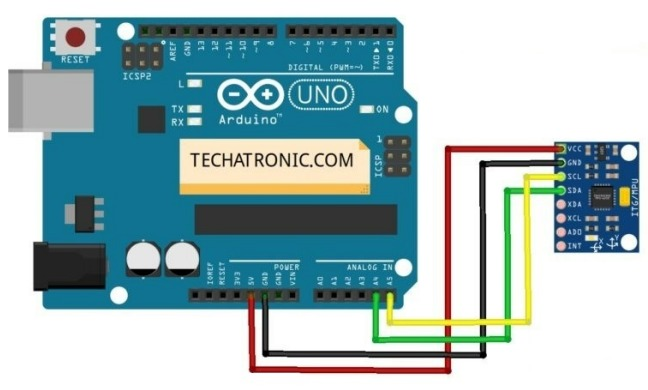
\includegraphics[width=0.4\textwidth]{figures/setup.jpeg}}
    \caption{MPU-6050 and Arduino UNO setup for this project.}
    \label{fig: setup}
\end{figure}

The Arduino code provided for this problem accompanies this report and also is attached in the appendix. This Arduino code reads data from the MPU-6050 sensor using the DMP (Digital Motion Processor) to obtain yaw, pitch, and roll angles.\cite{b4} \\

\subsection{To summarize the program briefly:}
\begin{enumerate}
    \item The code initializes the sensor and the serial communication for output.
    \item It checks the connection to the MPU-6050 sensor.
    \item The DMP is initialized, and if successful, it's enabled to start reading data from the sensor.
    \item Inside the main loop:
          \begin{itemize}
              \item It reads a packet from the FIFO buffer.
              \item If the flag {\texttt{OUTPUT\_READABLE\_QUATERNION}} is defined, it obtains the quaternion values $(w, x, y, z)$ and prints them to the serial monitor.
              \item If the flag {\texttt{OUTPUT\_READABLE\_YAWPITCHROLL}} is defined, it obtains the yaw, pitch, and roll angles from the quaternion values and prints them to the serial monitor.
          \end{itemize}
\end{enumerate}

The yaw, pitch, and roll angles are obtained using the quaternion values and gravity vector. These angles represent the orientation of the sensor in space relative to a fixed reference frame. The code then converts these angles from radians to degrees for readability.

Overall, this code demonstrates how to utilize the DMP functionality of the MPU-6050 sensor to obtain orientation data in the form of yaw, pitch, and roll angles. After that, the results are taken to the \textbf{Serial Plotter} application\cite{b6} to visually show the angles alter by rotating the setup.


\subsection{To explain the program precisely:}

\subsubsection{Library Inclusions}

The code starts by including necessary libraries for communicating with the MPU-6050 sensor and processing its data. These libraries include \texttt{"I2Cdev.h"} for I2C communication, \texttt{"MPU6050\_6Axis\_MotionApps20.h"} for working with the MPU6050's DMP, and \texttt{"Wire.h"} for I2C communication on Arduino platforms.\\

\subsubsection{Global Variables}

Global variables such as \texttt{mpu}, \texttt{q}, \texttt{gravity}, \texttt{ypr}, and \texttt{dmpReady} are declared. These variables are used throughout the code to interface with the MPU6050 sensor and store sensor data.\\

\subsubsection{Setup Function}

The \texttt{setup()} function initializes the serial communication, sets the I2C clock speed, and initializes the MPU6050 sensor. It then checks the connection to the MPU6050 sensor and initializes the DMP. If the DMP initialization is successful, it enables the DMP, indicating that the sensor is ready to start reading data.\\

\subsubsection{Loop Function}

The \texttt{loop()} function continuously runs in a loop once the setup is complete. Inside the loop, it checks if the DMP is ready. If not, it exits the loop. It reads a packet from the FIFO buffer using \texttt{mpu.dmpGetCurrentFIFOPacket(fifoBuffer)}. If the flag \texttt{OUTPUT\_READABLE\_QUATERNION} is defined, it obtains the quaternion values (w, x, y, z) from the packet and prints them to the serial monitor. If the flag \texttt{OUTPUT\_READABLE\_YAWPITCHROLL} is defined, it obtains the yaw, pitch, and roll angles from the quaternion values and prints them to the serial monitor.\\

\subsubsection{Quaternion and Yaw/Pitch/Roll Calculation}

The quaternion values represent the orientation of the sensor in 3D space. Yaw, pitch, and roll angles are calculated from these quaternion values using the \texttt{mpu.dmpGetYawPitchRoll()} function. Yaw, pitch, and roll angles are then converted from radians to degrees for readability using the formula \texttt{angle\_degrees = angle\_radians * 180 / PI}.\\

It's important to note that based on which of the two results the client wants to see (Quaternion or Yaw/Pitch/Roll), one of the two variables introduced at the beginning of the code must be defined and the other one commented. There are also two commented sections in the \textit{setup} block. Since our sensor was placed on the breadboard upside down, these sections mislead the result, so they're commented out.
\vspace{10px}






\section{Problem 2: Angle Filtering}
Digital filters are essential components in control systems used to process and manipulate signals for effective control. They play a crucial role in achieving stability, performance, and reliability in modern control systems.
A digital filter is a system that performs mathematical operations on a sampled, discrete-time signal to reduce or enhance certain aspects of that signal. In signal processing, the function of a filter is to remove unwanted parts of the signal, such as random noise, or to extract useful parts of the signal, such as the components lying within a certain frequency range. There are two main kinds of filters: analog and digital. They are quite different in their physical makeup and in how they work.

\subsection{First Order Complementary Filter}
A First Order Complementary Filter is a type of sensor fusion algorithm commonly used to combine data from multiple sensors, typically an accelerometer and a gyroscope, to estimate the orientation or motion of an object.\\

\subsubsection{Overview}
The basic idea behind a complementary filter is to blend the noisy, high-frequency data from one sensor (typically the gyroscope) with the stable, low-frequency data from another sensor (typically the accelerometer) to produce a more accurate and stable estimate of the object's orientation or motion.

In a First Order Complementary Filter, the output is a weighted combination of the raw sensor data and the filtered data from the previous timestep. The blending of the two signals is achieved using a simple first-order low-pass filter. This filter attenuates the high-frequency components of the gyroscope data while preserving the low-frequency components of the accelerometer data.

The blending parameter, often denoted as $\alpha$, determines the amount of influence each sensor's data has on the final estimate. It is typically chosen based on the relative noise levels and bandwidths of the sensors. A smaller $\alpha$ value gives more weight to the gyroscope data, resulting in faster response to changes in orientation but more noise, while a larger $\alpha$ value gives more weight to the accelerometer data, resulting in smoother but slower response.

The output of the complementary filter provides an estimation of the orientation or motion of the object, which can be used in various applications such as robotics, drones, and virtual reality systems.\\

\subsubsection{Formula}
The output of a First Order Complementary Filter, often denoted as \( \theta_{\text{filter}} \), is typically calculated as a weighted sum of the raw sensor data \( \theta_{\text{gyro}} \) (from a gyroscope) and the filtered data \( \theta_{\text{accel}} \) (from an accelerometer). The formula for the output can be expressed as:

\[ \theta_{\text{filter}} = \alpha \cdot \theta_{\text{gyro}} + (1 - \alpha) \cdot \theta_{\text{accel}} \]

where:
\begin{itemize}
    \item \( \theta_{\text{gyro}} \) is the raw data from the gyroscope (angular velocity),
    \item \( \theta_{\text{accel}} \) is the filtered data from the accelerometer (orientation),
    \item \( \alpha \) is the blending parameter (\( 0 \leq \alpha \leq 1 \)), which determines the influence of the gyroscope data relative to the accelerometer data.
\end{itemize}

% \vspace{2px}

This formula represents a simple linear combination of the gyroscope and accelerometer data, where the gyroscope data is weighted by \( \alpha \) and the accelerometer data is weighted by \( (1 - \alpha) \). The value of \( \alpha \) is typically chosen based on the characteristics of the sensors and the requirements of the specific application.

Overall, a First Order Complementary Filter offers a simple and effective way to combine data from different sensors to improve the accuracy and stability of orientation or motion estimation. However, it may require tuning of the blending parameter $\alpha$ to achieve optimal performance for specific applications and sensor configurations.

\subsection{Kalman Filter}

The Kalman filter is an algorithm used for estimating the state of a linear dynamic system from a series of noisy measurements. It is widely used in various fields such as engineering, navigation, robotics, finance, and signal processing.\\

\subsubsection{Overview}

The Kalman filter maintains an estimate of the current state of the system, including both the state variables (e.g., position, velocity) and their uncertainties (covariance matrix). It predicts the state of the system at the next timestep based on the previous estimate and the system dynamics, accounting for the uncertainty associated with the system dynamics. When new measurements become available, it updates the state estimate by combining the predicted state with the new measurements, considering their uncertainties (measurement noise). The Kalman filter iterates between prediction and update steps, refining the state estimate as new measurements are received.\\

\subsubsection{Optimal Fusion}

The Kalman filter performs a weighted fusion of the prediction and measurement information to obtain an optimal estimate of the current state. The weights are determined based on the relative uncertainties of the prediction and measurements (covariance matrices).\\

\subsubsection{Extensions}

Extensions of the Kalman filter, such as the Extended Kalman Filter (EKF) and Unscented Kalman Filter (UKF), allow for the estimation of non-linear systems by linearizing or approximating the system dynamics and measurement models. \\


The Kalman filter is a versatile and widely used tool for state estimation and sensor fusion in various applications. Its efficiency, optimality, and robustness make it a cornerstone algorithm in the field of estimation and control.

\subsection{Implementation}
To implement the mentioned filters on the outputs of the previous problem, an Arduino code is provided which accompanies this report and is also attached in the appendix. This program implements a sensor fusion algorithm using both a Kalman filter\cite{b7}\cite{b8} and a complementary filter to estimate the orientation (roll and pitch angles) of an object using data from an accelerometer and a gyroscope; so the \textit{quaternions} are erased from the program flow.\\

\subsubsection*{Explanation of the Code}
This code has the same structure as the one for previous problem; only it has some modifications like:
\begin{itemize}
    \item Some new variables are defined related to the 2 filters and their outputs. Also a new block is added to implement the filters.
    \item The \texttt{updateFiltered()} function is called periodically to update the filtered orientation angles.
    \item It calculates the time interval \texttt{dt} between successive function calls using the \texttt{micros()} function, which measures the current time in microseconds.
    \item The roll and pitch angles are calculated using the arctangent function (\texttt{atan2()}) based on the accelerometer readings (\texttt{ax}, \texttt{ay}, \texttt{az}). These angles are converted from radians to degrees.
    \item The raw gyroscope readings (\texttt{gx}, \texttt{gy}, \texttt{gz}) are converted to degrees per second (\texttt{gyroXrate}, \texttt{gyroYrate}, \texttt{gyroZrate}) by dividing by the sensitivity factor (\texttt{131.0})\footnote{In fact, the data we get by \texttt{mpu.getRotation(\&gx, \&gy, \&gz);} is gyroscope's very raw and meaningless output. It must be scaled by a number which depends on the Sensor type and is mentioned in its catalog. For the sensor possessed in this project, the scale factor was $131.0$. That's what lines 58 to 60 are for.}.
    \item The Kalman filter is applied to estimate the roll and pitch angles based on the gyroscope and accelerometer data. If the angles exceed a certain threshold (-90° to 90°), the Kalman filter is reset to the accelerometer reading to prevent abrupt changes.
    \item The complementary filter combines the gyroscope and accelerometer data to estimate the roll and pitch angles (\texttt{compAngleX} and \texttt{compAngleY}). It uses a weighted sum of the gyroscope-derived angle change (\texttt{gyroXrate * dt}, \texttt{gyroYrate * dt}) and the accelerometer-derived angle (\texttt{roll} and \texttt{pitch}). The weights (\texttt{0.80} and \texttt{0.20}) determine the contribution of each sensor to the final estimate.
    \item To address transition problems when the accelerometer angle jumps between -180° and 180°, the Kalman filter is reset to the accelerometer reading.
    \item The previous angle values (\texttt{ang\_x\_prev} and \texttt{ang\_y\_prev}) are updated for use in the next iteration.
    \item The \texttt{setup()} function is almost the same as before, except it does some initializations of variables related to the filters at its end.
    \item The \texttt{loop()} function is also the same as it was in problem 1, except it runs \texttt{updateFiltered()} function and prints its results for a better comparison of the filters and the raw data.
\end{itemize}


\subsection{Comparison between Raw Data and Filtered Data}
By observing the changes of the \textit{Yaw}, \textit{Pitch} and \textit{Roll} angles in \textbf{raw} outputs, \textbf{Complementary filter} outputs and \textbf{Kalman filter} outputs, we can reach an important estimation of the algorithms. It can be seen that raw data has quite much delay than the filtered results. In fact, by rotating the sensor, the raw data takes a long time to converge to the actual value of angles, while the filters speed up this procedure quite tangibly. Another difference is the fluctuations of the results. Unlike filtered outputs, raw angles fluctuate a lot around their actual values. Their oscillations sometimes reach beyond a range of \(10^\circ-15^\circ\) error. The filtered angles, on the other hand, have less than \(1^\circ\) of error.

\subsection{Comparison between Complementary and Kalman Filters}
This project was too simple to distinguish the results of the two filters. Both of them, as a matter of fact, worked quite admissibly; however, it is known that in general, complementary filter is simpler and lighter but Kalman filter is more accurate and robust. A concise comparison between Kalman and complementary filters can be seen below:
\begin{enumerate}
    \item \textbf{Accuracy}:
          \begin{itemize}
              \item \textbf{Kalman Filter:} Provides optimal estimates, especially in dynamic environments and with Gaussian noise.
              \item \textbf{Complementary Filter:} Offers simpler estimates, may lack optimality, and may struggle with non-linearities or significant sensor noise.
          \end{itemize}

    \item \textbf{Robustness}:
          \begin{itemize}
              \item \textbf{Kalman Filter:} Robust to noise and uncertainties, adapts well to changing conditions.
              \item \textbf{Complementary Filter:} Less robust, may require manual tuning and struggle with changing sensor characteristics.
          \end{itemize}

    \item \textbf{Computational Complexity}:
          \begin{itemize}
              \item \textbf{Kalman Filter:} More computationally intensive, suitable for real-time processing but may require efficient implementations.
              \item \textbf{Complementary Filter:} Simple and computationally efficient, ideal for resource-constrained systems.
          \end{itemize}

    \item \textbf{Implementation Complexity}:
          \begin{itemize}
              \item \textbf{Kalman Filter:} Requires understanding of mathematics and parameter tuning.
              \item \textbf{Complementary Filter:} Easier to implement and understand, minimal parameter tuning required.
          \end{itemize}

    \item \textbf{Applicability}:
          \begin{itemize}
              \item \textbf{Kalman Filter:} Versatile, suitable for various systems and sensors, especially in applications requiring optimal state estimation.
              \item \textbf{Complementary Filter:} Suited for simple systems and resource-limited applications, commonly used in low-cost sensor fusion applications.
          \end{itemize}
\end{enumerate}
\vspace{10px}





\section{Problem 3: MPU-6050 as a Game Controller}
In this Problem, we use the knowledge from previous problems to turn our sensor into a game controller. To lead the avatar throughout the maze to find its destination, we utilize the sensor's orientation. By rotating the sensor about two axes, its \underline{Roll} and \underline{Pitch} angles alter and make the avatar go Left/Right or Forward/Backward. To do so, an Arduino program is needed to read the pitch \& roll angles, at the same time as a python code generating and executing the game. The Arduino is loaned from the previous problem, except that its raw data and complementary filter are eradicated. That's because \underline{Kalman filter} proved to be the best of them for the highly sensitive burden a game controller must carry. It should also be mentioned that we only expect to get \textit{pitch} and \textit{roll} angles from this code, because the \textit{maze game} we intend to control is 2-dimensional and doesn't need the third angle.\\

The \textit{Python} code is derived from the provided code in the problem\cite{b5}. To complete and customize the program several changes has been made to the code; some of its most important modifications are:
\begin{itemize}
    \item The \textbf{serial} module is imported to connect Arduino to this code.
    \item Frame rate of the game is set to \(60 fps\).
    \item Serial communication is initialized with Arduino by ``ser = serial.Serial('com3', 115200)'' command.
    \item The data from MPU-6050 sensor is read through serial communication, within the \textit{Game loop}.
    \item It is checked to ensure that the captured data is indeed a <two index number>; this helps ignoring the string (text) outputs of the Arduino code.
    \item The angles are interpreted to left/right and forward/backward directions based on two range of $(30^\circ, 170^\circ)$ and $(-170^\circ, 30^\circ)$
    \item Player's position is adjusted by replacing "W-A-S-D" keys by the obtained directions to move the ball.
\end{itemize}
\vspace{5px}
Both Python code and Arduino code for this problem are accessible alongside this document and attached to its appendix.
\vspace{10px}





\section{Problem 4: Motion Capturing Using MediaPipe}
Motion capturing with AI involves using artificial intelligence algorithms and techniques to track and analyze human motion from video or sensor data. AI-based motion capture systems can automatically detect and interpret movements in real-time or from recorded footage, enabling applications in fields such as animation, sports analysis, healthcare, and virtual reality.

\subsection{Overview}
One tool for motion capturing with AI is MediaPipe, an open-source framework developed by Google. MediaPipe provides pre-trained models and pipelines for various tasks, including human pose estimation, hand tracking, and facial recognition. It offers efficient and accurate solutions for extracting key points or landmarks from video streams, allowing developers to build custom motion capture applications or integrate motion tracking capabilities into their projects \cite{b9}.

In this problem, we recorded a short random movement of a person's leg and used MediaPipe to track its ankle and knee, so that we can find the angles of its rotation. As explained in the problem's description, due to the inaccuracy of MediaPipe in depth estimation, we had to record the motion from both lateral and frontal view of the leg simultaneously. Afterwards we needed to read the videos in a Python code and extract each of its frames to hand it over to MediaPipe AI model to process it \cite{b10}.

\subsection{Procedures}
The greatest challenge was that we wanted the videos to start together, exactly at the same time, and stop in the same manner \cite{b11}. Only in this way we could be sure that each frame of one video is corresponding to the same frame of the other video. We had to ensure both cameras recorded the video with the same FPS so both videos could have the same length. To achieve these, a third party application was used to pre-process the videos before handing it over to the code. With \textbf{\textit{BandiCut}} application, both videos were opened at the same time and conformity of their corresponding frames were adjusted manually by cutting the videos at precise frames. Nevertheless, since this procedure was operated by human vision, it might not be $100\%$ flawless, but it satisfies the purpose. using 4 heat maps of knee and ankle positions and comparing them with the recorded video, the accuracy of the code is examined and approved. The results can be seen in Figure~\ref{fig:heat}.

With the fixed coordinate system shown in  Figure~\ref{fig:coordinates}, the angles $\theta_x$ and $\theta_y$ of one's leg can be measured by knowing the coordinates of two points from one's leg which are its knee and ankle. This is what MediaPipe is supposed to tell us. After that, using $\arctan(\frac{\sin}{\cos})$ both angles are found. Additionally, the $\theta_z$ is known to be zero since the leg does not have any rotation about $Z$ axis. 

\begin{figure}[htbp]
  \centerline{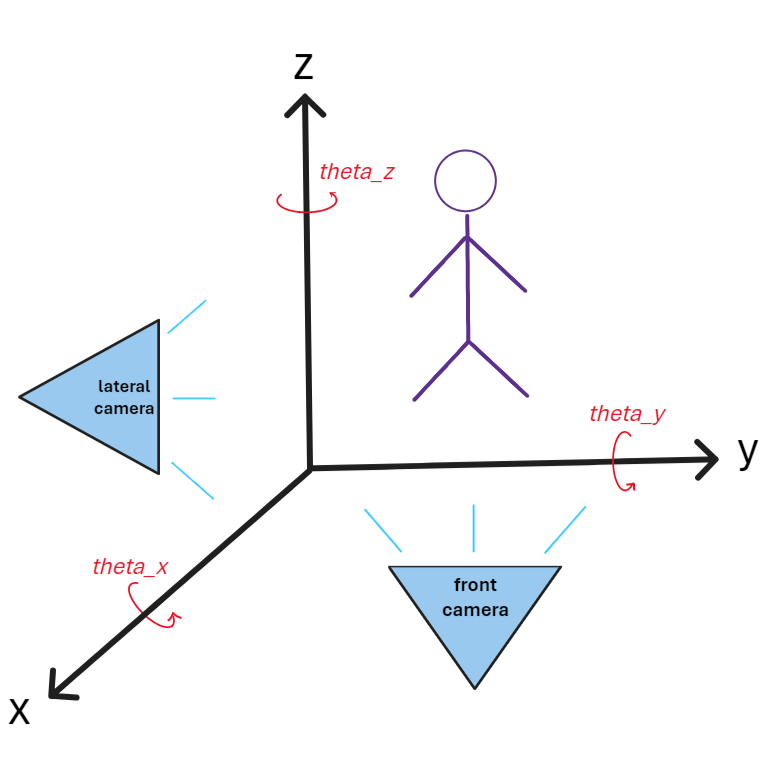
\includegraphics[width=0.4\textwidth]{figures/coordinates.png}}
  \caption{Global coordinate system and Recording setup}
  \label{fig:coordinates}
\end{figure}

The rotation matrix then is formed for each set of angles found in each frame. From the reference text book \cite{b2}, the rotation matrix for a fixed origin system that implies to rotating $\theta_x$ degrees about $x$, $\theta_y$ degrees about $y$, and $\theta_z$ degrees about $z$ axes is introduced as below. Note that with this deceleration, $\theta_x$, $\theta_y$ and $\theta_z$ imply to \textbf{Roll}, \textbf{Pitch} and \textbf{Yaw} respectively.

\begin{align}
  &R_{xyz}(\theta_x, \theta_y, \theta_z) = \\
  &\begin{bmatrix}
    c\theta_z c\theta_y & c\theta_z s\theta_y s\theta_x - s\theta_z c\theta_x & c\theta_z s\theta_y c\theta_x + s\theta_z s\theta_x \\
    s\theta_z c\theta_y & s\theta_z s\theta_y s \theta_x + c \theta_z  c \theta_x & s \theta_z s \theta_y c \theta_x -	c \theta_z s \theta_x \\
    -s\theta_y & c \theta_y s \theta_x & c \theta_y c\theta_x
  \end{bmatrix} \nonumber
\end{align} \\

Then the vector \( \vec{\mathbf{e}} \) and the quaternion value is derived from each rotation matrix using the equations \ref{eq:phi}, \ref{eq:e} and \ref{eq:r0}. The quaternion value is then plotted and shown in Figure~\ref{fig:Q}

\begin{align}
  &\text{Angle of rotation: } \phi = \cos ^{-1} \left(\frac{tr(\mathbf{R}) - 1}{2}\right) \label{eq:phi} \\
  &\text{Axis of rotation: } \mathbf{e} = \frac{\text{vect}(\mathbf{R})}{\sin \phi}       \label{eq:e} \\
  &\text{Quaternion value: } r_0 = \cos \frac{\phi}{2}  \label{eq:r0}
\end{align}

Afterwards, the obtained series of $\theta_x$ and $\theta_y$ are plotted and shown in Figure~\ref{fig:angles}. It's observed that the sharp edges of the plot might resemble the effect of noises. To smoothen it out, a \textbf{Moving Average Smoothening} is applied to the plots in Python. Moving average smoothing is a technique used to reduce noise and remove short-term fluctuations in time series data. It involves replacing each data point with the average of itself and its neighboring points within a specified window or interval. Here's how moving average smoothing works in our program: \\

\begin{enumerate}
    \item \textbf{Choose a Window Size}: Determine the size of the window or interval over which the moving average will be calculated. This window size represents the number of adjacent data points used in the smoothing process. The choice of window size is crucial and depends on the characteristics of the data and the level of smoothing desired. A larger window size provides more smoothing but may obscure rapid changes in the data, while a smaller window size retains more detail but may not effectively filter out noise.
    
    \item \textbf{Compute the Moving Average}: For each data point in the original series, calculate the average value of itself and its neighboring points within the window. This average value becomes the smoothed value for that data point.
    
    \item \textbf{Handling Boundary Cases}: At the edges of the data series where there are not enough neighboring points to form a complete window, various approaches can be used, such as padding or truncating the data.
    
    \item \textbf{Apply the Smoothing}: Once the moving average has been computed for each data point, the resulting smoothed series can be plotted or used for further analysis.
\end{enumerate}

Moving average smoothing is effective at reducing noise and revealing the underlying trend or pattern in the data, especially for long-term trends. However, it can also introduce a lag or delay, particularly with larger window sizes, as the smoothed data reflects the average behavior over the window interval. \\

By re-plotting the results, it can be seen (Figure~\ref{fig:filter}) that the noises are truncated with the smoothening process implemented. These noises might have come from the inaccuracy of MediaPipe in locating the coordinates of knee and ankle, inconformity of frames from both videos, lack of clearness and low resolution of some frames of the videos, round-off errors of the computer, and etc.

\subsection{Results}

\begin{figure}[H]
  \centering
  \includegraphics[width=0.4\textwidth]{figures/figure_1.png}
  \includegraphics[width=0.4\textwidth]{figures/figure_2.png}
  \includegraphics[width=0.4\textwidth]{figures/figure_3.png}
  \includegraphics[width=0.4\textwidth]{figures/figure_4.png}
  \caption{Heat Maps of knee and ankle positions}
  \label{fig:heat}
\end{figure}

\begin{figure}[htbp]
  \centering
  \includegraphics[width=0.4\textwidth]{figures/figure_5.png}
  \includegraphics[width=0.4\textwidth]{figures/figure_6.png}
  \caption{Raw outputs of rotation angles with respect to time}
  \label{fig:angles}
\end{figure}

\begin{figure}[htbp]
  \centering
  \includegraphics[width=0.4\textwidth]{figures/figure_8.png}
  \includegraphics[width=0.4\textwidth]{figures/figure_9.png}
  \caption{Comparison of Raw and Filtered rotation angles}
  \label{fig:filter}
\end{figure}

\begin{figure}[htbp]
  \centering
  \includegraphics[width=0.4\textwidth]{figures/figure_7.png}
  \caption{Quaternion value with respect to time}
  \label{fig:Q}
\end{figure}


\section{Conclusion}
\textbf{
    As a conclusion, our exploration into the four problems revealed significant insights. Angle Recording: The MPU-6050 provides accurate angle measurements, but calibration and noise reduction are crucial. Future work should focus on optimizing its performance.
    Angle Filtering: Implementing effective filters enhances stability and responsiveness. Researchers can explore adaptive filters and fusion techniques.
    Game Controller Application: Integrating the MPU-6050 into gaming systems offers exciting possibilities. Fine-tuning its responsiveness and compatibility is essential.
    MediaPipe for Motion Capturing: MediaPipe shows promise in real-time motion analysis. Further research should address scalability and robustness.
    In summary, our project contributes to robotics advancements, emphasizing precision, efficiency, and interdisciplinary collaboration.
}

\vspace{30px}
\begin{thebibliography}{00}

  \bibitem{b1} J. Angeles, ``Fundamentals of Robotic Mechanical Systems'', Theory, Methods, and Algorithms, 4th edition, Springer.

  \bibitem{b2} J. J. Craig, ``Introduction to Robotics'', 3d edition, Pearson Education, Inc.

  \bibitem{b3} Hamilton, W.R., 1844, ``On quaternions: or a new system of imaginaries in algebra'', Phil. Mag., 3rd. ser. 25, pp. 489-495.

  \bibitem{b4} P. Namazian, ``Mechatronics-and-Robotics-Mini-Project'', Github, \url{https://github.com/Parsanmz/Mechatronics-and-Robotics-Mini-Project}

  \bibitem{b5} S. Kazemi, ``Robotics Course TA'', Github, \url{https://github.com/Sinakzm1379/Robotics_Course_TA/}

  \bibitem{b6} H. Y. Özderya, ``SerialPlot - Realtime Plotting Software'', \url{https://hackaday.io/project/5334-serialplot-realtime-plotting-software}

  \bibitem{b7} K. Lauszus, ``Kalman Filter Library'', TKJ Electronics, Arduino.cc, \url{https://www.arduino.cc/reference/en/libraries/kalman-filter-library/}

  \bibitem{b8} R. JL. Fetick, ``Kalman: Implement Kalman filter for your Arduino projects'', Github, \url{https://github.com/rfetick/Kalman}

  \bibitem{b9} Google for Developers, ``Pose landmark detection guide'', 2024-01-23 UTC, \url{https://developers.google.com/mediapipe/solutions/vision/pose_landmarker}

  \bibitem{b10} J. Fernandez, ``MediaPipe Pose'', Github \url{https://github.com/google/mediapipe/blob/master/docs/solutions/pose.md}

  \bibitem{b11} PyPI, ``mediapipe 0.10.11'', MediaPipe, 2024-03-06, \url{https://pypi.org/project/mediapipe/}

\end{thebibliography}
\vspace{80px}


% =============================================================
\section{Appendix}
\subsection{Arduino code for problem 1}

\begin{lstlisting}[style=Arduino]
#include "I2Cdev.h"

#include "MPU6050_6Axis_MotionApps20.h"

#if I2CDEV_IMPLEMENTATION == I2CDEV_ARDUINO_WIRE
#include "Wire.h"
#endif

MPU6050 mpu;


// uncomment "OUTPUT_READABLE_QUATERNION" if you want to see the actual
// quaternion components in a [w, x, y, z] format
#define OUTPUT_READABLE_QUATERNION

// uncomment "OUTPUT_READABLE_YAWPITCHROLL" if you want to see the yaw/
// pitch/roll angles (in degrees) calculated from the quaternions coming
// from the FIFO.
// #define OUTPUT_READABLE_YAWPITCHROLL

bool dmpReady = false;
uint8_t devStatus;
uint8_t fifoBuffer[64];

Quaternion q;         // [w, x, y, z]         quaternion container
VectorFloat gravity;  // [x, y, z]            gravity vector
float ypr[3];         // [yaw, pitch, roll]   yaw/pitch/roll container and gravity vector


void setup() {
#if I2CDEV_IMPLEMENTATION == I2CDEV_ARDUINO_WIRE
  Wire.begin();
  Wire.setClock(400000);
#elif I2CDEV_IMPLEMENTATION == I2CDEV_BUILTIN_FASTWIRE
  Fastwire::setup(400, true);
#endif

  Serial.begin(115200);
  while (!Serial)
    ;

  Serial.println(F("Initializing I2C devices..."));
  mpu.initialize();

  Serial.println(F("Testing device connections..."));
  Serial.println(mpu.testConnection() ? F("MPU6050 connection successful") : F("MPU6050 connection failed"));

  Serial.println(F("Initializing DMP..."));
  devStatus = mpu.dmpInitialize();
  /*
    mpu.setXGyroOffset(220);
    mpu.setYGyroOffset(76);
    mpu.setZGyroOffset(-85);
    mpu.setZAccelOffset(1788); 
    */
  if (devStatus == 0) {
    /*
        mpu.CalibrateAccel(6);
        mpu.CalibrateGyro(6);
        mpu.PrintActiveOffsets();
        */
    Serial.println(F("Enabling DMP..."));
    mpu.setDMPEnabled(true);

    dmpReady = true;
  } else {
    Serial.print(F("DMP Initialization failed (code "));
    Serial.print(devStatus);
    Serial.println(F(")"));
  }
}

void loop() {
  if (!dmpReady) return;
  // read a packet from FIFO
  if (mpu.dmpGetCurrentFIFOPacket(fifoBuffer)) {
#ifdef OUTPUT_READABLE_QUATERNION
    // display quaternion values in easy matrix form: w x y z
    mpu.dmpGetQuaternion(&q, fifoBuffer);
    Serial.print(q.w);
    Serial.print(",");
    Serial.print(q.x);
    Serial.print(",");
    Serial.print(q.y);
    Serial.print(",");
    Serial.println(q.z);
#endif

#ifdef OUTPUT_READABLE_YAWPITCHROLL
    // display Euler angles in degrees
    mpu.dmpGetQuaternion(&q, fifoBuffer);
    mpu.dmpGetGravity(&gravity, &q);
    mpu.dmpGetYawPitchRoll(ypr, &q, &gravity);
    float roll = ypr[2] * 180 / M_PI;
    float pitch = ypr[1] * 180 / M_PI;
    float yaw = ypr[0] * 180 / M_PI;
    Serial.print(roll);  // roll
    Serial.print(",");
    Serial.print(pitch);  // pitch
    Serial.print(",");
    Serial.println(yaw);  // yaw
#endif
  }
}
\end{lstlisting}

% =============================================================
\subsection{Arduino code for problem 2}

\begin{lstlisting}[style=Arduino]
#include "I2Cdev.h"
#include <Kalman.h>
#include "MPU6050_6Axis_MotionApps20.h"


#if I2CDEV_IMPLEMENTATION == I2CDEV_ARDUINO_WIRE
#include "Wire.h"
#endif

// uncomment "OUTPUT_READABLE_QUATERNION" if you want to see the actual
// quaternion components in a [w, x, y, z] format
//#define OUTPUT_READABLE_QUATERNION

// uncomment "OUTPUT_READABLE_YAWPITCHROLL" if you want to see the yaw/
// pitch/roll angles (in degrees) calculated from the quaternions coming
// from the FIFO.
#define OUTPUT_READABLE_YAWPITCHROLL

// Variables related to gyroscope data
bool dmpReady = false;
uint8_t devStatus;
uint8_t fifoBuffer[64];

Quaternion q;         // [w, x, y, z]         quaternion container
VectorFloat gravity;  // [x, y, z]            gravity vector
float ypr[3];         // [yaw, pitch, roll]   yaw/pitch/roll container and gravity vector

// Variables related to complementary filter data
int ax, ay, az;
int gx, gy, gz;

long tiempo_prev;
float dt;
float ang_x_prev, ang_y_prev;

// Variables related to kalman filter data
Kalman kalmanX;  // Create the Kalman instances
Kalman kalmanY;
int16_t tempRaw;

double compAngleX, compAngleY;  // Calculated angle using a complementary filter
double kalAngleX, kalAngleY;    // Calculated angle using a Kalman filter


const int mpuAddress = 0x68;  // It can be 0x68 or 0x69
MPU6050 mpu(mpuAddress);


void updateFiltered() {
  // Calculate the execution time of the function in each round
  dt = (micros() - tiempo_prev) / 1000000.0;
  tiempo_prev = micros();

  //Calculate the angles with accelerometer
  float roll = atan2(ay, az) * (180.0 / M_PI);
  float pitch = atan2(ax, az) * (180.0 / M_PI);

  double gyroXrate = gx / 131.0;  // Convert to deg/s
  double gyroYrate = gy / 131.0;  // Convert to deg/s
  double gyroZrate = gz / 131.0;  // Convert to deg/s

  if ((roll < -90 && kalAngleX > 90) || (roll > 90 && kalAngleX < -90)) {
    kalmanX.setAngle(roll);
    compAngleX = roll;
    kalAngleX = roll;
  } else {
    kalAngleX = kalmanX.getAngle(roll, gyroXrate, dt);  // Calculate the angle using a Kalman filter
  }

  if (abs(kalAngleX) > 90) {
    gyroYrate = -gyroYrate;  // Invert rate, so it fits the restriced accelerometer reading
  }
  kalAngleY = kalmanY.getAngle(pitch, gyroYrate, dt);

  // This fixes the transition problem when the accelerometer angle jumps between -180 and 180 degrees
  if ((pitch < -90 && kalAngleY > 90) || (pitch > 90 && kalAngleY < -90)) {
    kalmanY.setAngle(pitch);
    compAngleY = pitch;
    kalAngleY = pitch;
  } else {
    kalAngleY = kalmanY.getAngle(pitch, gyroYrate, dt);  // Calculate the angle using a Kalman filter
  }

  if (abs(kalAngleY) > 90) {
    gyroXrate = -gyroXrate;  // Invert rate, so it fits the restriced accelerometer reading
  }
  kalAngleX = kalmanX.getAngle(roll, gyroXrate, dt);  // Calculate the angle using a Kalman filter

  //Calculate rotation angle with gyroscope and complementary filter
  compAngleX = 0.80 * (ang_x_prev + gyroXrate * dt) + 0.20 * roll;
  compAngleY = 0.80 * (ang_y_prev + gyroYrate * dt) + 0.20 * pitch;

  ang_x_prev = compAngleX;
  ang_y_prev = compAngleY;
}


void setup() {

  delay(1000);  // Wait for sensor to stabilize
  Serial.begin(115200);
  Wire.begin();
#if I2CDEV_IMPLEMENTATION == I2CDEV_ARDUINO_WIRE
  Wire.setClock(400000);
#elif I2CDEV_IMPLEMENTATION == I2CDEV_BUILTIN_FASTWIRE
  Fastwire::setup(400, true);
#endif

  while (!Serial)
    ;

  Serial.println(F("Initializing I2C devices..."));
  mpu.initialize();

  Serial.println(F("Testing device connections..."));
  Serial.println(mpu.testConnection() ? F("MPU6050 connection successful") : F("MPU6050 connection failed"));

  Serial.println(F("Initializing DMP..."));
  devStatus = mpu.dmpInitialize();
  /*
  mpu.setXGyroOffset(220);
  mpu.setYGyroOffset(76);
  mpu.setZGyroOffset(-85);
  mpu.setZAccelOffset(1788); 
  */
  if (devStatus == 0) {
    /*
    mpu.CalibrateAccel(6);
    mpu.CalibrateGyro(6);
    mpu.PrintActiveOffsets();
    */
    Serial.println(F("Enabling DMP..."));
    mpu.setDMPEnabled(true);
    dmpReady = true;
  } else {
    Serial.print(F("DMP Initialization failed (code "));
    Serial.print(devStatus);
    Serial.println(F(")"));
  }

  // complementary and kalman filter
  mpu.initialize();
  // calculate roll and pitch angle as primary data
  float roll = atan2(mpu.getAccelerationY(), mpu.getAccelerationZ()) * (180.0 / M_PI);
  float pitch = atan2(mpu.getAccelerationX(), mpu.getAccelerationZ()) * (180.0 / M_PI);
  // Set starting angle
  kalmanX.setAngle(roll);
  kalmanY.setAngle(pitch);
  ang_x_prev = roll;
  ang_y_prev = pitch;
}

void loop() {
  if (!dmpReady) return;
  // read a packet from FIFO
  if (mpu.dmpGetCurrentFIFOPacket(fifoBuffer)) {
#ifdef OUTPUT_READABLE_QUATERNION
    // display quaternion values in easy matrix form: w x y z
    mpu.dmpGetQuaternion(&q, fifoBuffer);
    Serial.print(q.w);
    Serial.print(",");
    Serial.print(q.x);
    Serial.print(",");
    Serial.print(q.y);
    Serial.print(",");
    Serial.println(q.z);
#endif

#ifdef OUTPUT_READABLE_YAWPITCHROLL
    mpu.dmpGetQuaternion(&q, fifoBuffer);
    mpu.dmpGetGravity(&gravity, &q);
    mpu.dmpGetYawPitchRoll(ypr, &q, &gravity);
    float roll = ypr[2] * 180 / M_PI;
    float pitch = ypr[1] * 180 / M_PI;
    float yaw = ypr[0] * 180 / M_PI;
    Serial.print("Gyroscope data| ");
    Serial.print("Roll: ");
    Serial.print(roll);  // roll
    Serial.print(", ");
    Serial.print("Pitch: ");
    Serial.print(pitch);  // pitch
    Serial.print(", ");
    Serial.print("Yaw: ");
    Serial.print(yaw);  // yaw
    Serial.print("\t\t");
#endif
  }

  // Read accelerations and angular velocities
  mpu.getAcceleration(&ax, &ay, &az);
  mpu.getRotation(&gx, &gy, &gz);


  // Use complementary and kalman filter
  updateFiltered();

  // Print roll and pitch angle with complementary and kalman filter
  Serial.print("complementary filter data| ");
  Serial.print("Roll: ");
  Serial.print(compAngleX);
  Serial.print(", ");
  Serial.print("Pitch: ");
  Serial.print(compAngleY);
  Serial.print("\t\t");
  Serial.print("Kalman filter data| ");
  Serial.print("Roll: ");
  Serial.print(kalAngleX);
  Serial.print(", ");
  Serial.print("Pitch: ");
  Serial.print(kalAngleY);
  Serial.print("\r\n");

  delay(10);
}

\end{lstlisting}

% =============================================================
\subsection{Arduino code for problem 3}

\begin{lstlisting}[style=Arduino]
#include "I2Cdev.h"
#include <Kalman.h>
#include "Wire.h"
#include "MPU6050_6Axis_MotionApps20.h"

// Variables related to complementary filter data
int ax, ay, az;
int gx, gy, gz;

long tiempo_prev;
float dt;

// Variables related to kalman filter data
// Create the Kalman instances
Kalman kalmanX;
Kalman kalmanY;

// for calculate time
int16_t tempRaw;

double kalAngleX, kalAngleY;  // Calculated angle using a Kalman filter


const int mpuAddress = 0x68;  // It can be 0x68 or 0x69
MPU6050 mpu(mpuAddress);


void updateFiltered() {
  // Calculate the execution time of the function in each round
  dt = (micros() - tiempo_prev) / 1000000.0;
  tiempo_prev = micros();

  //Calculate the angles with accelerometer
  float roll = atan2(ay, az) * (180.0 / M_PI);
  float pitch = atan2(-ax, az) * (180.0 / M_PI);

  double gyroXrate = gx / 131.0;  // Convert to deg/s
  double gyroYrate = gy / 131.0;  // Convert to deg/s
  double gyroZrate = gz / 131.0;  // Convert to deg/s

  if ((roll < -90 && kalAngleX > 90) || (roll > 90 && kalAngleX < -90)) {
    kalmanX.setAngle(roll);
    kalAngleX = roll;
  } else {
    kalAngleX = kalmanX.getAngle(roll, gyroXrate, dt);  // Calculate the angle using a Kalman filter
  }

  if (abs(kalAngleX) > 90) {
    gyroYrate = -gyroYrate;  // Invert rate, so it fits the restriced accelerometer reading
  }
  kalAngleY = kalmanY.getAngle(pitch, gyroYrate, dt);

  // This fixes the transition problem when the accelerometer angle jumps between -180 and 180 degrees
  if ((pitch < -90 && kalAngleY > 90) || (pitch > 90 && kalAngleY < -90)) {
    kalmanY.setAngle(pitch);
    kalAngleY = pitch;
  } else {
    kalAngleY = kalmanY.getAngle(pitch, gyroYrate, dt);  // Calculate the angle using a Kalman filter
  }

  if (abs(kalAngleY) > 90) {
    gyroXrate = -gyroXrate;  // Invert rate, so it fits the restriced accelerometer reading
  }
  kalAngleX = kalmanX.getAngle(roll, gyroXrate, dt);  // Calculate the angle using a Kalman filter
}


void setup() {
  delay(1000);  // Wait for sensor to stabilize
  Serial.begin(115200);
  Wire.begin();
  // complementary and kalman filter
  mpu.initialize();
  // calculate roll and pitch angle as primary data
  float roll = atan2(mpu.getAccelerationY(), mpu.getAccelerationZ()) * (180.0 / M_PI);
  float pitch = atan2(-mpu.getAccelerationX(), mpu.getAccelerationZ()) * (180.0 / M_PI);
  // Set starting angle
  kalmanX.setAngle(roll);
  kalmanY.setAngle(pitch);
}

void loop() {
  // Read accelerations and angular velocities
  mpu.getAcceleration(&ax, &ay, &az);
  mpu.getRotation(&gx, &gy, &gz);


  // Use complementary and kalman filter
  updateFiltered();

  // Print roll and pitch angle with kalman filter
  Serial.print(kalAngleX);
  Serial.print(",");
  Serial.print(kalAngleY);
  Serial.print("\r\n");

  delay(10);
}

\end{lstlisting}

% =============================================================
\subsection{Python code for problem 3}

\begin{lstlisting}[language=Python]
# Libraries
import pygame
import sys
import serial
import time
import random

# Initialize Pygame
pygame.init()

# Constants
WIDTH, HEIGHT = 600, 600
CELL_SIZE = 30
ROWS, COLS = HEIGHT // CELL_SIZE, WIDTH // CELL_SIZE
FPS = 60  # Adjust the FPS for slower movement

# Colors
WHITE = (255, 255, 255)
GRAY = (181, 176, 173)
DARK_BLUE = (3, 102, 150)
MEDIUM_BLUE = (7, 87, 91)
LIGHT_BLUE = (173, 216, 230)
RED = (255, 0, 0)

# Initialize clock
clock = pygame.time.Clock()

# Initialize serial communication with Arduino
ser = serial.Serial("com3", 115200)


# Maze generation - DO NOT CHANGE THIS FUNCTION!
def generate_maze():
    maze = [[0] * COLS for _ in range(ROWS)]
    stack = []
    start_cell = (1, 1)
    end_cell = (ROWS - 3, COLS - 3)
    stack.append(start_cell)
    maze[start_cell[0]][start_cell[1]] = 1

    while stack:
        current_cell = stack[-1]
        neighbors = [
            (current_cell[0] - 2, current_cell[1]),
            (current_cell[0] + 2, current_cell[1]),
            (current_cell[0], current_cell[1] - 2),
            (current_cell[0], current_cell[1] + 2),
        ]
        unvisited_neighbors = [
            neighbor
            for neighbor in neighbors
            if 0 < neighbor[0] < ROWS - 1
            and 0 < neighbor[1] < COLS - 1
            and maze[neighbor[0]][neighbor[1]] == 0
        ]

        if unvisited_neighbors:
            chosen_neighbor = random.choice(unvisited_neighbors)
            maze[chosen_neighbor[0]][chosen_neighbor[1]] = 1
            maze[(chosen_neighbor[0] + current_cell[0]) // 2][
                (chosen_neighbor[1] + current_cell[1]) // 2
            ] = 1
            stack.append(chosen_neighbor)
        else:
            stack.pop()

    return maze, start_cell, end_cell


maze, start_point, end_point = generate_maze()

# Player position
player_row, player_col = start_point

# Initialize the screen
screen = pygame.display.set_mode((WIDTH, HEIGHT))
pygame.display.set_caption("Maze Game")


# Game loop
while True:
    for event in pygame.event.get():
        if event.type == pygame.QUIT:
            pygame.quit()
            sys.exit()

    # Read data from Arduino through serial communication
    data = ser.readline().decode().strip().split(",")
    if len(data) == 2:
        roll, pitch = map(float, ser.readline().decode().strip().split(","))
        # Map roll and pitch to player movement
        if 30 < roll < 170:
            if player_col > 0 and maze[player_row][player_col - 1] == 1:
                player_col -= 1
        elif -170 < roll < -30:
            if player_col < COLS - 1 and maze[player_row][player_col + 1] == 1:
                player_col += 1
        if 30 < pitch < 170:
            if player_row > 0 and maze[player_row - 1][player_col] == 1:
                player_row -= 1
        elif -170 < pitch < -30:
            if player_row < ROWS - 1 and maze[player_row + 1][player_col] == 1:
                player_row += 1

    # Draw maze
    screen.fill(WHITE)
    for row in range(ROWS):
        for col in range(COLS):
            if maze[row][col] == 1:
                pygame.draw.rect(
                    screen,
                    MEDIUM_BLUE,
                    (col * CELL_SIZE, row * CELL_SIZE, CELL_SIZE, CELL_SIZE),
                )
    for row in range(ROWS):
        for col in range(COLS):
            if (row, col) == start_point:
                pygame.draw.rect(
                    screen,
                    LIGHT_BLUE,
                    (col * CELL_SIZE, row * CELL_SIZE, CELL_SIZE, CELL_SIZE),
                )
            elif (row, col) == end_point:
                pygame.draw.rect(
                    screen,
                    LIGHT_BLUE,
                    (col * CELL_SIZE, row * CELL_SIZE, CELL_SIZE, CELL_SIZE),
                )

    # Draw player
    pygame.draw.circle(
        screen,
        GRAY,
        (
            player_col * CELL_SIZE + CELL_SIZE // 2,
            player_row * CELL_SIZE + CELL_SIZE // 2,
        ),
        CELL_SIZE // 3,
    )

    # Check if the player reaches the end point
    if (player_row, player_col) == end_point:
        pygame.display.flip()
        print("Congratulations! You reached the end of the maze.")
        time.sleep(5)
        pygame.quit()
        sys.exit()

    pygame.display.flip()
    clock.tick(FPS)

\end{lstlisting}

% =============================================================
\subsection{Python code for problem 4}

\begin{lstlisting}[language=Python]
import cv2
import mediapipe as mp
import math
import sys
import matplotlib.pyplot as plt
from matplotlib.colors import LinearSegmentedColormap
import numpy as np

# Initialize MediaPipe Pose
mp_pose = mp.solutions.pose
pose = mp_pose.Pose()

# Open the video files by cv2
video_path_1 = 'E:/w1.mp4'  # front view video file location
video_1 = cv2.VideoCapture(video_path_1)
video_path_2 = 'E:/w2.mp4'  # Sideview video file location
video_2 = cv2.VideoCapture(video_path_2)

# Check if the videos opened successfully
if not video_1.isOpened():
    print("Error! Could not open the video1!")
    sys.exit(0)
if not video_2.isOpened():
    print("Error! Could not open the video2!")
    sys.exit(0)

RightAnkleY_1 = []
RightAnkleZ_1 = []
RightKneeY_1 = []
RightKneeZ_1 = []
my_theta_x = []

RightAnkleX_2 = []
RightAnkleZ_2 = []
RightKneeX_2 = []
RightKneeZ_2 = []
my_theta_y = []

Q, phi, e, r, r0 = [], [], [], [], []


def rotation_matrix(alpha, beta):
    R = np.array([[np.cos(beta), np.sin(beta)*np.sin(alpha), np.sin(beta)*np.cos(alpha)],
                  [0, np.cos(alpha), -np.sin(alpha)],
                  [-np.sin(beta), np.cos(beta)*np.sin(alpha), np.cos(beta)*np.cos(alpha)]])
    return R


def vect(R):
    return (1/2 * np.array([[R[2, 1]-R[1, 2]], [R[0, 2]-R[2, 0]], [R[1, 0]-R[0, 1]]]))


while True:
    # Read frames
    ret_1, frame_1 = video_1.read()
    ret_2, frame_2 = video_2.read()

    # if the videos end, break
    if not ret_1 and not ret_2:
        break

    # Convert frame to RGB
    frame_1 = cv2.cvtColor(frame_1, cv2.COLOR_BGR2RGB)
    frame_2 = cv2.cvtColor(frame_2, cv2.COLOR_BGR2RGB)

    height1, width1 = frame_1.shape[0], frame_1.shape[1]
    height2, width2 = frame_2.shape[0], frame_2.shape[1]

    # Process with MediaPipe Pose
    result_1 = pose.process(frame_1)
    result_2 = pose.process(frame_2)

    if result_1.pose_landmarks:
        y_right_knee_1 = (
            result_1.pose_landmarks.landmark[mp_pose.PoseLandmark.RIGHT_KNEE].x
            * frame_1.shape[1]
        )
        z_right_knee_1 = (
            frame_1.shape[0]
            - result_1.pose_landmarks.landmark[mp_pose.PoseLandmark.RIGHT_KNEE].y
            * frame_1.shape[0]
        )
        y_right_ankle_1 = (
            result_1.pose_landmarks.landmark[mp_pose.PoseLandmark.RIGHT_ANKLE].x
            * frame_1.shape[1]
        )
        z_right_ankle_1 = (
            frame_1.shape[0]
            - result_1.pose_landmarks.landmark[mp_pose.PoseLandmark.RIGHT_ANKLE].y
            * frame_1.shape[0]
        )

        RightAnkleY_1.append(y_right_ankle_1)
        RightAnkleZ_1.append(z_right_ankle_1)
        RightKneeY_1.append(y_right_knee_1)
        RightKneeZ_1.append(z_right_knee_1)

        z = z_right_knee_1 - z_right_ankle_1
        y = y_right_knee_1 - y_right_ankle_1
        L = math.sqrt(y**2 + z**2)
        th_x_rad = math.atan2(z / L, y / L)
        th_x_deg = math.degrees(th_x_rad)
        my_theta_x.append(th_x_deg)  # theta_x

    if result_2.pose_landmarks:
        x_right_knee_2 = (
            result_2.pose_landmarks.landmark[mp_pose.PoseLandmark.RIGHT_KNEE].x
            * frame_2.shape[1]
        )
        z_right_knee_2 = (
            frame_2.shape[0]
            - result_2.pose_landmarks.landmark[mp_pose.PoseLandmark.RIGHT_KNEE].y
            * frame_2.shape[0]
        )
        x_right_ankle_2 = (
            result_2.pose_landmarks.landmark[mp_pose.PoseLandmark.RIGHT_ANKLE].x
            * frame_2.shape[1]
        )
        z_right_ankle_2 = (
            frame_2.shape[0]
            - result_2.pose_landmarks.landmark[mp_pose.PoseLandmark.RIGHT_ANKLE].y
            * frame_2.shape[0]
        )

        RightAnkleX_2.append(x_right_ankle_2)
        RightAnkleZ_2.append(z_right_ankle_2)
        RightKneeX_2.append(x_right_knee_2)
        RightKneeZ_2.append(z_right_knee_2)

        z = z_right_knee_2 - z_right_ankle_2
        x = x_right_knee_2 - x_right_ankle_2
        L = math.sqrt(x**2 + z**2)
        th_y_rad = math.atan2(z / L, x / L)
        th_y_deg = math.degrees(th_y_rad)
        my_theta_y.append(th_y_deg)  # theta_y

    Q.append(rotation_matrix(th_x_rad, th_y_rad))
    phi.append(np.arccos((np.trace(Q[-1])-1)/2))
    e.append(vect(Q[-1])/np.sin(phi[-1]))   # vector e
    r.append(e[-1]*np.sin(phi[-1]/2))
    r0.append(np.cos(phi[-1]/2))    # quaternion value
    print(f"frame {len(Q)}:\te={e[-1].reshape(1, 3)},\t r0={r0[-1]}")


# Release videos
video_1.release()
video_2.release()

numFrames = len(Q)
seconds = numFrames / 30
print('\nfront view frames:\t width =', width1, 'height =', height1)
print('side view frames:\t width =', width2, 'height =', height2)
print('\nnumber of frames processed:', numFrames)
print('length of videos in seconds:', round(seconds, 4))


# Defining some functions to simplify the plotting processes

def posPlot(X, Y, w, h, name):
    # Define the colormap from green to red
    colors = [(0, 'green'), (0.5, 'yellow'), (1, 'red')]
    cmap = LinearSegmentedColormap.from_list('CustomCmap', colors)

    # Compute the color gradient based on the position of points
    gradient = [(j / numFrames) for j in range(numFrames)]

    # Plotting the points with color gradient
    plt.title(name)
    plt.scatter(X, Y, c=gradient, cmap=cmap, s=10)
    plt.xlim(0, w)
    plt.ylim(0, h)

    # Customizing colorbar
    cbar = plt.colorbar()
    cbar.set_ticks([0, 0.5, 1])
    cbar.set_ticklabels(['Start', '', 'Stop'])

    plt.grid()
    plt.show()


def angPlot(angle, name):
    X = np.arange(0, seconds, 1/30)
    plt.title(rf"{name}")
    plt.plot(X, angle)
    if not 'r_0' in name:
        plt.ylim(0, 200)
        plt.ylabel('degrees')
    plt.xlabel('seconds')
    plt.grid()
    plt.show()


def smoothPlot(angle, name):
    X = np.arange(0, seconds, 1/30)

    # Applying moving average smoothing
    window_size = 6
    y_smooth = np.convolve(angle, np.ones(
        window_size)/window_size, mode='valid')

    plt.plot(X[window_size//2:-window_size//2+1],
             y_smooth, label='Filtered', color='r')
    plt.plot(X, angle, label='Raw', color='b', alpha=0.6)

    plt.title(rf"{name}")
    plt.xlabel('seconds')
    plt.ylabel('degrees')
    plt.grid()
    plt.legend()
    plt.show()


# Drawing the plots
posPlot(RightKneeX_2, RightKneeZ_2, width2, height2, 'Right Knee Side view')
posPlot(RightAnkleX_2, RightAnkleZ_2, width2, height2, 'Right Ankle Side view')
posPlot(RightKneeY_1, RightKneeZ_1, width1, height1, 'Right Knee Front view')
posPlot(RightAnkleY_1, RightAnkleZ_1, width2,
        height2, 'Right Ankle Front view')

angPlot(my_theta_x, "Roll angle (front view): $\\theta_x$")
angPlot(my_theta_y, "Pitch angle (side view): $\\theta_y$")
angPlot(r0, 'Quternion Value $r_0$:')
smoothPlot(my_theta_x, "Filtered Roll angle: $\\theta_x$")
smoothPlot(my_theta_y, "Filtered Pitch angle: $\\theta_y$")

\end{lstlisting}

% =============================================================

\end{document}
